\colorlet{chaptergrey}{black}
%\renewcommand*\sectfont{\color{orange}}
\chapter[Discrete dynamical models of stacked dark matter haloes]{Galaxies as potential tracers: \\ Discrete dynamical models of stacked dark matter haloes in IllustrisTNG}
\label{ch:dyn_mod}
\vspace{-5.25in}
\includegraphics[height=1.18in]{thesis/latex/headers/cw_left.pdf}
\vspace{3in}

%\epigraph{Eat slugs malfoy.}

\section{Introduction}
In the framework of the cosmic web, matter flows preferentially from under-dense to over-dense regions under the influence of the gravitational potential of the cosmic web. In Figure \ref{fig:disperse_matter_path}, we show a diagram of the flow of matter of the cosmic web, using morphological features identified by DisPerSE in IllustrisTNG300. As large-scale structure grows, material is sucked out of voids from the walls that in-case them. These walls are framed by filaments, so that matter travels along walls into the filaments, perpendicular to the filament's major axis. Once in the reference frame of the filament, material moves along its major axis, towards maxima (nodes; galaxy groups or clusters). Numerical simulations show that the natural anisotropy of the cosmic web imprints distinct signatures in the orbits of material accreting onto dark matter haloes. Haloes forming at these intersections (saddle) points should experience large degrees of anisotropy since matter is collapsing perpendicular to the filament from the walls but is moving to more dense regimes (nodes) along the direction of the filament itself \citep[e.g.][for galaxy properties in saddle environments]{kraljic2019saddle}. Outside the immediate influence of the cosmic web, lower mass dark matter halos should be able to continue to form matter more isotropically. The decrease in the tidal field strength enables the halos to continue accreting material from smaller scale filamentary structure, leading to more radial orbits.

\begin{figure*}
    \centering
	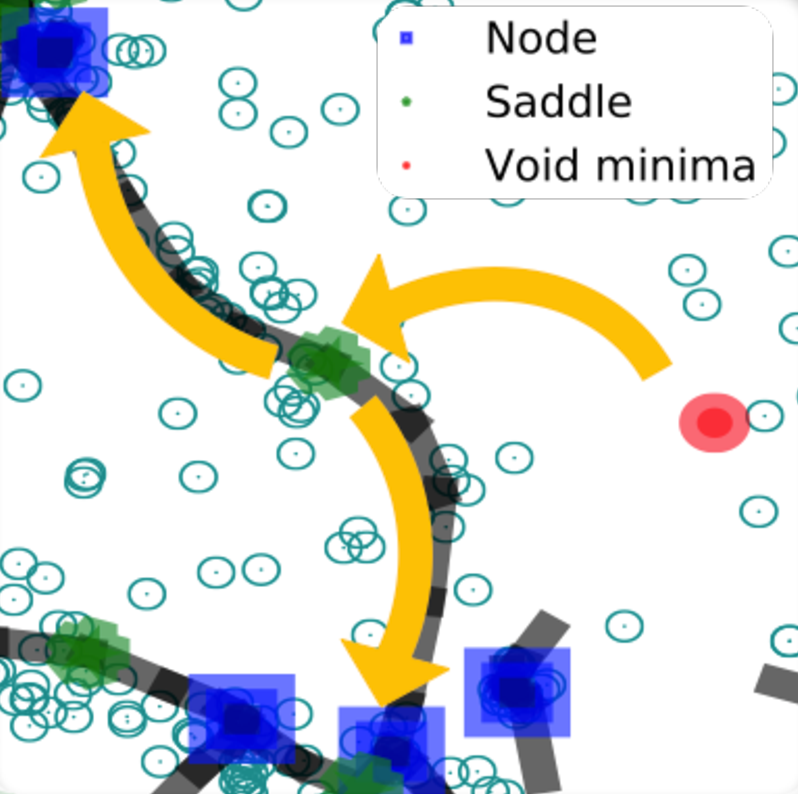
\includegraphics[width=0.5\linewidth]{thesis/latex/dyn_mod_files/disperse_matter_path.pdf}
    \caption{Representation of the flow of matter in large-scale structure. The empty green circles show the galaxy distribution in a slice of IllustrisTNG300 from which DisPerSE has been applied to. Identified nodes (blue squares), saddle points (green stars) and minima (red circles) are shown with filaments (black lines). The yellow arrows show the flow of matter to hierarchically higher mass environments. Mass is sucked out of voids which are funnelled into filaments through walls. Once within filaments, matter moves preferentially along the plane of the filament to the most over-dense regimes: nodes (galaxy groups or clusters). This flow of material inwards (perpendicular) and outwards (parallel) to a given point in the plane of the filament, creates the anisotropy we see in orbits of dark matter; \textit{especially} in saddle points.}
    \label{fig:disperse_matter_path}
\end{figure*}

In numerical simulations, the degree of perturbation from pure isotropic radial accretion is quantified by velocity anisotropy (ratio between velocity moments in tangential and radial directions). This is typically calculated by considering the total population of dark matter particles associated with the halo. On this basis, the orbits have greater tangential dispersion in haloes within environments of both higher tidal field strength and over-density \citep[e.g.][]{faltenbacher2010, shi2015}. Tidal field strength is innately related to the cosmic web, however, making a direct link to how this is modulated by filamentary structure and saddle points individually is difficult. 

Baryonic matter is also subject to the gravitational potential of the cosmic web, and, to first order, should trace the same orbits as seen in the dark matter. \citep[][]{garaldi2018} demonstrate this through considering the orbits of all satellite galaxies (albeit including those below the typical mass observable in redshift surveys) within milky way sized haloes. Satellites in those haloes embedded in (or in close vicinity to) large filamentary structure, display distinctly more anisotropic orbits, than those in isolated haloes. Being able to trace the anisotropy though satellite galaxies is promising for observations, however, recovering 3D motions for galaxies is extremely difficult.

In this chapter, we aim to trace the flow of dark matter near different morphological features of the cosmic web, through using satellite galaxies as tracers. In particular, we are interested in the impact of large scale structure on low mass dark matter haloes ($\mathrm{M_{DM} \sim 10^{12}M_{\odot}}$), whose evolution is modulated most strongly by large scale tidal fields, and hence, most likely to trace the anistropy of the cosmic web \citep[e.g.][]{tojeiro2017}. This brings an additional difficulty, as these low mass haloes will host low numbers of satellite galaxies. Using the cosmological simulation of IllustrisTNG300, we stack low mass haloes in different cosmic web environments (voids, saddle points, and filaments) to recover the difference in velocity anisotropy. To consider the dynamics within each environment we require $\sim$1000 so we stack in consistent regimes while maintaining orientation and scaling characteristic group lengths. We use this study to motivate the potential to recover the 3D motions of satellites in observations through a new application of the axisymmetric Jeans equations, and hence, the velocity anisotropy of the environment they trace. In section \S\ref{sec:dyn_mod_aniso}, we introduce the data, methodology, and results associated with using satellites galaxies as tracers in different cosmic web environments in IllustrisTNG. In section \S\ref{sec:jam}, we introduce the basics and methodology of discrete dynamical modelling, and highlight the potential for it to be used to recover 3D satellite galaxy dynamics in observations. We also present a re-derivation of the axis-symmetric jeans equations to include gravitational collapse, and removing the steady state assumption. Finally we summarise our findings and conclude in \S\ref{sec:dyn_mod_conclusions}.

\section{Anisotropy in the cosmic web} \label{sec:dyn_mod_aniso}
\subsection{Data}
\subsubsection{IllustrisTNG300}
Throughout this chapter, we base our analysis on galaxies selected from the 300Mpc box of the IllustrisTNG simulation suite. Nominally referred to as IllustrisTNG300 (TNG300), this simulation run follows the evolution of 2500$^3$ dark matter particles ($\mathrm{M_{DM} = 4 x 10^{7}h^{-1}M_{\odot}}$) and 2500$^3$ gas cells ($\mathrm{M_{gas} = 7.6 x 10^{6}h^{-1}M_{\odot}}$. The prescriptions for baryonic physics are consistent with TNG100 (see \S\ref{sec:sim_data_TNG} for further details), however TNG300 provides a far larger cosmological volume, at the cost of spatial resolution.

\subsubsection{Galaxy sample} \label{sec:gal_samp}
In parallel with TNG100, gravitationally bound structures in TNG300 are identified into haloes and subhaloes through use of a friends-of-friends algorithm \citep{davis85} and the subfind algorithm \citep{springel01} respectively (see \S\ref{sec:sim_data_TNG}). In this work, we select a galaxy sample in TNG300 by considering all $z=0$ (snapshot 99) subhaloes which contain a minimum stellar mass of $\mathrm{M_{\ast} = 10^{8} M_{\odot}}$ within a 3D aperture of 30 comoving kpc from the subhalo centre \citep[as defined in;][]{pillepich18b}. This corresponds to 564,930 unique galaxies which we use for both reconstruction of the cosmic web, and for the satellite tracers in the velocity anisotropy calculations.

In the context of halo assembly, we are particularly interested in isolating the impact of the cosmic web on low mass dark matter haloes. To this effect, we select all galaxies (from our sample above) that reside in a FoF halo of mass $\mathrm{10^{11.5} M_{\odot} < M_{h} < 10^{12.5} M_{\odot}}$, which we use to stack in each cosmological environment as described in \S\ref{sec:stacking}. 

\subsubsection{Cosmological environment}
To identify morphological features of the cosmic web, we make use of DisPerSE (see \S\ref{sec:cosmic_web_intro} for more information). We apply DisPerSE directly to the spatial distribution of our selected galaxy sample in the periodic cube of TNG300. In Figure \ref{fig:disperse_TNG300}, we show the spatial distribution of galaxies for a 10Mpc slice through TNG300, along with the identified filamentary network from DisPerSE.

\begin{figure*}
	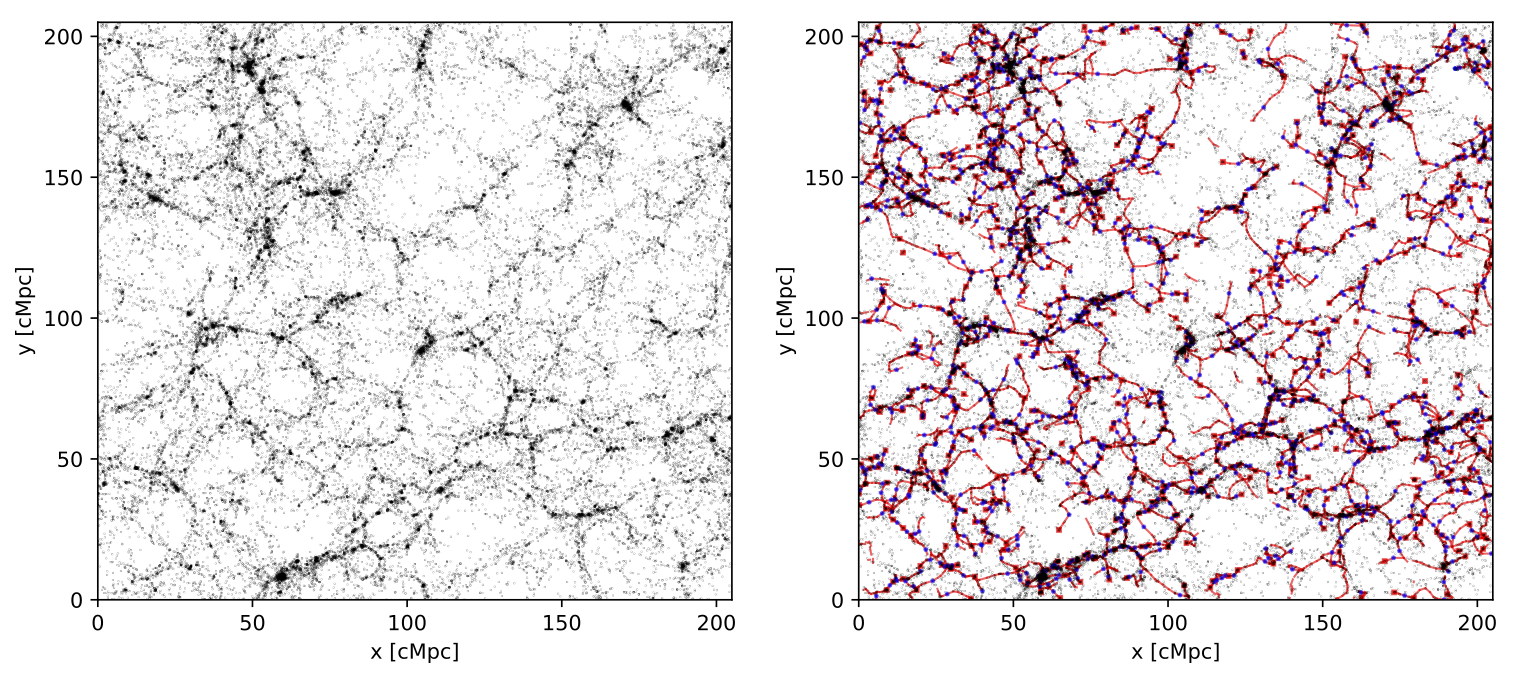
\includegraphics[width=\linewidth]{dyn_mod_files/TNG300-1-SM10-8-slice-galaxy-density-skeleton-comparison.png}
    \caption{Illustration of the filamentary network identified from galaxy positions within a 10 Mpc slice in TNG. The left panel shows the distribution of galaxy ($\mathrm{M_{\ast} > 10^{8}M_{\odot}}$) positions within the slice. The right panel shows the same but with filamentary structure overlaid (red lines). Critical points are also shown such as nodes (red squares) and saddle points (blue stars) highlighting the ensemble which the skeleton connects.}
    \label{fig:disperse_TNG300}
\end{figure*}

Having constructed a skeleton of the cosmic web, we now look to classify the selected haloes into distinct cosmological environments. In similarity with \S\ref{sec:cosmic_web_distances}, for each FoF halo (computed from the centre point), the distance to the nearest node ($\mathrm{D_{node}}$), filament segment ($\mathrm{D_{skel}}$) and saddle point ($\mathrm{D_{2-saddle}}$) is found. 

\subsubsection{Stacking of cosmic web environments} \label{sec:stacking}
In order to trace the differences in orbits for different cosmic web environments with satellite galaxies, we need enough tracers to first compute the anisotropy directly, and further, enough to test the feasibility of recovering the anisotropy through dynamical models in observations. Since our focus is on the impact on low mass haloes, we only have a handful (at best) of satellite galaxies to use as tracers. To proceed, we therefore must stack similar haloes in the same topological environment. 

For each environment (node, filament, saddle point) we select all galaxies in FoF haloes with $\mathrm{10^{11.5} M_{\odot} < M_{h} < 10^{12.5} M_{\odot}}$. To ensure we are only selecting FoF haloes that are only subject to a certain morphological feature and hence remove effects due to the proximity of other environments, we take all those within the following conservative selections as shown in Table \ref{tab:stacking}. 

\begin{table}
\centering
\begin{tabular}{|l|c|c|c|}
\hline
& Filament & 2-saddle & Void \\ \hline
$D_{node}$ & > 2 Mpc & > 2 Mpc & > 5 Mpc \\
$D_{skel}$ & < 0.5 Mpc  & - - & > 5 Mpc \\
$D_{2-saddle}$ & > 1 Mpc & < 0.75 Mpc & > 5 Mpc \\
Number of galaxies: & 8071 & 941 & 2246 \\
\hline
\end{tabular}
\caption{Selection criteria for stacks in three different environments; filaments, 2-saddle points and voids. Each row shows the distance cut used to select an environment apart from the final row which shows the total number of galaxies selected.}
\label{tab:stacking}
\end{table}

In addition to the distribution of satellites, we also require an assumed dark matter potential for each stacked environment. To construct a reliable dynamical model, all tracers should reside in gravitational potentials that are consistent in overall mass and scale. For every FoF halo that contains a galaxy to be stacked we take the density profile and scale it according to the characteristic group scale as defined by $R_{200}$ (comoving radius of a sphere centered on the FoF halo whose mean density is 200 times the critical density of the Universe). The magnitude of the density profile is scaled according to the total mass contained in the FoF halo and then combined so that each stacked density profile contributes equally to the final profile. The stacked FoF halo density profile is finally scaled so that its total mass is equal to the median for the stacked population. We then convert the final density profile to the gravitational potential as described in \ref{sec:grav_pot}. Each tracer position and velocity is also scaled by the characteristic group scale of its host FoF halo, $\mathrm{R_{200}}$. \red{Should velocity be scaled according to mass or is this accounted for by the scale?}. 

A natural assumption of the axis-symmetric Jeans equations is symmetry around the principal axis of rotation, and hence, it is important to retain directionality while stacking tracers (galaxies) and potentials. In the instance of saddle points and filaments, we use the direction of the nearest filament segment (from saddle to node) to stack galaxy positions/velocities and the gravitational potential around. For those stacked far away from large scale structure (i.e. voids), we use the direction of the overall angular momentum vector of the dark matter in the central subhalo.

\subsection{Velocity anisotropy} \label{sec:velocity_anisotropy}
\subsubsection{Results}
For each environment stack, we first directly compute the anisotropy from the three-dimensional motions of the satellite galaxies. We define two measures of anisotropy, based on the radial and tangential velocity moments. Following \citet{faltenbacher2010}, we refer to the \textit{velocity anisotropy parameter} as such;
\begin{equation} \label{eq:vel_ani_sigma}
\mathrm{\beta_{\sigma}(r) = 1 - \frac{\sigma_t^2(r)}{\sigma_r^2(r)} }
\end{equation}
where $\sigma_r^2(r)$ and $\sigma_t^2(r)$ denote the radial and tangential velocity dispersions. Additionally, we also compute the \textit{satellite anisotropy parameter}, motivated in \citet{ZOMGiii} to compute the anisotropy directly from the orbits of satellite subhaloes. This is defined as follows,
\begin{equation}
\beta_{sat}(r) = 1 - \frac{v_{t}^2(r)}{v_{r}^{2}(r)} 
\end{equation}
where $v_{t}(r)$ and $v_{r}(r)$ denote the radial and tangential velocities.

In Figure \ref{fig:beta_stack}, we show the radial profiles of both $\beta_{sat}$ (left) and $\beta_{\sigma}$ (right) for all satellites in each environment stack. The radial profiles are computed by a set of logarithmically spaced (in radial space) concentric shells, which range from 0 Mpc (from the stack centre, defined by the position of the central galaxy) to 1 Mpc. The number of radial bins are chosen to ensure a reliable measure of anistropy in each shell, which varies between stacks due to varying total numbers of tracers. In each panel we show the profiles for the void (red, dotted), filament (black, dot-dashed) and saddle (green, solid) stacks, accompanied by the average values (grey box) across all radii. 

\begin{figure}
	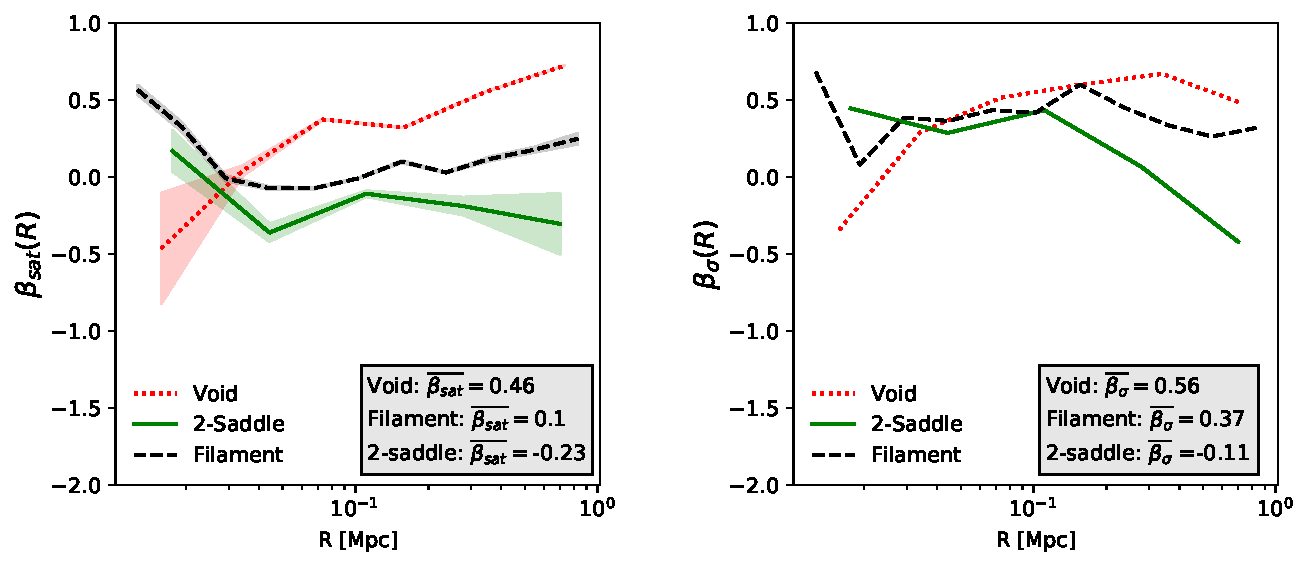
\includegraphics[width=\linewidth]{thesis/latex/dyn_mod_files/disperse_beta_paper.pdf}
    \caption{Velocity anisotropy profiles found from satellite galaxies in the void (red, dotted), filament (black, dot-dashed) and 2-saddle (green, solid) stacks. The left (right) panel corresponds to $\beta_{sat}$ ($\beta_{\sigma}$) with the shaded regions showing error on the mean. The average value for all satellites in each stack is shown in the grey box. For both $\beta_{sat}$ and $\beta_{\sigma}$, there is a clear distinction in orbital anisotropy between environments which increases with radii.}
    \label{fig:beta_stack}
\end{figure}

Starting with the left panel, we find that overall $\beta_{sat}$ is distinctly different between environments ranging from radially biased orbits (voids; positive $\beta_{sat}$) to tangentially biased orbits (saddles, negative $\beta_{sat}$) with intermediate orbits in filaments. As expected, the difference in anisotropy is far more distinct in the outer regions of the halo (i.e. $> 0.1$Mpc), where the impact of large scale tides can take hold over the driving force of the self-gravity of the halo. These differences are also reflected in the dispersions (right panel), where again saddle points host satellites that are on more tangentially biased orbits (particularly in their outer halo) with respect to voids, with orbits in filaments at intermediate values. In both instances, computing average values of orbital anisotropy we find distinct differences between environments. As discussed in \red{\S}, dynamical models require assumptions about the velocity anisotropy (as a parameter in the model). To reduce complexity in the model, it is often better to assume a flat profile in $beta_{\sigma}$, so it is promising that differences in anisotropy when considering the whole population average. It should be noted that while it is important to retain directionality in stacking for the purpose of dynamical modelling, it has no impact on the direct measures of $\beta_{\sigma}$ and $\beta_{sat}$.

\subsubsection{Discussion}
To interpret our findings, we now place these results in the context of previous studies making use of velocity anisotropy. On a particle level, the orbits within FoF haloes have been shown to be dependent on large scale environment. \citet{faltenbacher2010} used an implementation of the Tree-PM N-body code GADGET2 on-top of the Millenium simulation. They examine the correlation between clustering and halo properties such as shape, concentration, spin, shape of the velocity ellipsoid and velocity anisotropy ($\beta_{\sigma}$). They determine that $\beta_{\sigma}$ is most tightly correlated with the clustering strength, with halos of low velocity anisotropy being more highly clustered and the opposite holding true for haloes with strongly radially biased velocities. 

A possible explanation for more highly clustered haloes exhibiting a relatively larger tangential velocity dispersion is that the impact parameters of the merging sub-haloes are larger due to far more gravitational interactions a short time before accretion. This would lead to a greater dispersion of tangential velocities corresponding to a lower velocity anisotropy. On the other hand, in less clustered regions the gravitational field is dominated by the halo itself naturally leading to more radial in-fall. 

Velocity anisotropy has also been decomposed as a function of tidal environment. \cite{shi2015} investigate how halo dynamical properties are related to their formation histories and hence the tidal environment in which they reside. Figure \ref{fig:shifig11}, shows the relationship of $\beta_{\sigma}$ of particles in central `host' haloes and the tidal field strength in which these haloes reside. In both mass bins there is a clear correlation between $\beta_{\sigma}$ and the first eigenvalue of the tidal tensor (i.e. tidal field strength). As tidal field strength increases, $\beta_{\sigma}$ decreases, showing that again there is a greater dispersion in tangential orbits. 
\begin{figure}
\begin{center}
	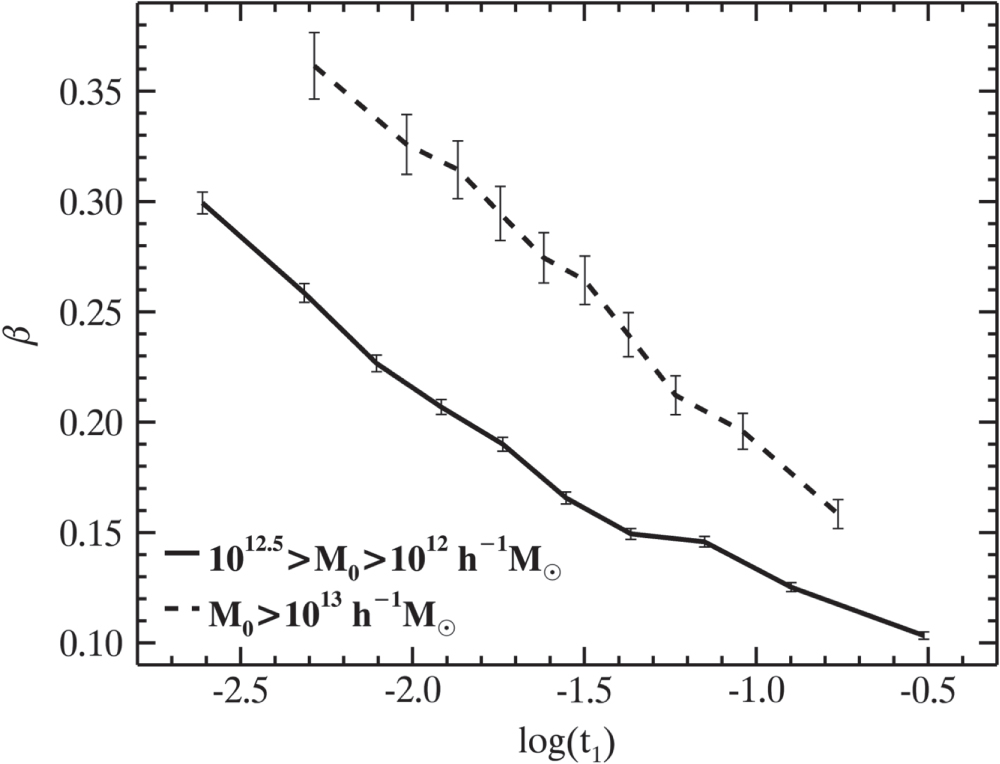
\includegraphics[width=0.5\linewidth]{thesis/latex/dyn_mod_files/shi2015fig11.jpg}
    \caption{Correlation between velocity anisotropy defined by equation \ref{eq:vel_ani_sigma} of host haloes and the first eigenvalue for the tidal field estimator. This plot is shows that as tidal field strength increases, $beta_{\sigma}$ decreases indicating more dispersion in tangential orbits.}
    \label{fig:shifig11}
\end{center}
\end{figure}

Extending this argument to include the impact of the cosmic web, the ZOMG (Zooming in On a Mob of Galaxies) paper series \cite{ZOMGI,ZOMGII,ZOMGiii}, present a set of zoom N-body and hydrodynamical simulations. They follow seven galaxy sized haloes selected on a definition of collapse time which generates strong assembly bias. These haloes are classified as `stalled' or accreting corresponding to the time at which their final mass becomes stable. Stalled haloes correspond to haloes which have become stable at $z \sim 1.5$ whereas accreting haloes are still yet to reach this point. 
The accreting haloes correspond with nodes of the cosmic web and are fed isotropically by radial infall of matter along thin filaments. Conversely `stalled' haloes are embedded in prominent filaments of the large-scale structure. Matter recedes along the filament to starve the early-forming halo as infall only becomes possible from the perpendicular directions. Overall this inflow is balanced by the outflow along the filament leading to no net mass growth. In this instance they follow the orbits on a satellite level rather than particle level. They find that the satellite anisotropy parameter at $z = 0$ is positive for accreting haloes and negative for stalled haloes showing that orbits become more tangentially biased (both in magnitude and dispersion) when low mass haloes are closer to large filamentary structure. Stalled haloes are also found to have a smaller fraction of their mass in sub-structure with respect to the accreting haloes. This can be see as a natural result of a more vibrant recent-accretion history for the later forming haloes. 

Our results are consistent with the idea of tidal forces acting to `stall' accretion leading to more tangentially biased orbits in the outskirts of haloes within filamentary structure. This effect is maximised in close vicinity to saddle points, due to the distinct anisotropy of material flowing in-wards perpendicular to the filament, and once accreted, preferentially along the filament. We show that satellite galaxies \textit{can} be used to trace the orbits within dark matter haloes, and distinct differences can be found between cosmic web environments. In the next section, we introduce the concept of discrete dynamical modelling in the context of the axis-symmetric Jeans equations, and consider the feasibility of applying them to observations, in order to recover their 3D motions, and hence velocity anisotropy.

\section{Potential applications of discrete dynamical models} \label{sec:jam}
Historically, the Jeans equations have served as a powerful tool to convert the observed projected luminosity distribution and kinematics of galaxies (or clusters of stars), to understand the underlying gravitational potential or the 3D de-projected kinematics. Under a series of assumptions, the Jeans equations enable best fitting models to understand further properties about the modelled system. In this section, we briefly introduce the Jeans equations under the assumption of axis-symmetry (\S\ref{sec:jeans_intro}), before re-deriving the equations removing the steady state assumption (\S\ref{sec:jeans_rederivation}). In \S\ref{sec:discrete_dynamical_models} we introduce the concept of dynamical models and motivate the usage in the context of satellite orbits, before summarising and concluding in \S\ref{sec:dyn_mod_conclusions}. 

\subsection{Introduction to the Jeans equations} \label{sec:jeans_intro}
The narrative in this section follows that of \citet{cappellari2008}, with additional explanation and context where necessary. The phase space distribution of positions ($x_{i}$) and velocities ($v_{i}$) for a set $i$ of tracers (such as stars, IFU spaxels or potentially satellite galaxies) within a massive system (such as a stellar cluster, galaxy or dark matter halo) can be characterised by the distribution function (DF): $f(x,v)$. If make the assumption that the system is in a \textit{steady state} (i.e. $\frac{\partial}{\partial t} = 0$: the system is not collapsing over time - we will return to this assumption later!) and the underlying gravitational potential ($\Phi$) that the tracers are subject to is smooth, then the DF \textit{must} satisfy the steady-state collisionless Boltzmann equation:
\begin{equation}
\sum^{3}_{i=1}\left(v_{i}\frac{\partial f}{\partial x_i} - \frac{\partial \Phi}{\partial x_{i}}\frac{\partial f}{\partial v_{i}} \right) = 0.
\end{equation}
Since $f$ is a function of 6 variables, there are quite a lot (infinite) of solutions to this equation, so to make use of this in a practical sense, we must make various assumptions. One method is to only consider the velocity moments of the DF; i.e. develop Jeans equations. 

\subsubsection{Some assumptions}
The first step in simplifying the solutions is to make use of the natural symmetry of the system. Common assumptions include spheroidal or axial symmetry, since dark matter haloes are often flattened (\red{reference?}), here we make use of the Jeans equations under the assumption of axis-symmetry. We can make our lives easier by transforming to cylindrical polar coordinates $(R,z,\phi)$. In the context of our stacked environments, this corresponds to the radial distance along the axis of stacking ($z$, i.e. direction of nearest filament or rotational axis), the radial distance perpendicular to this ($R$) and the rotation direction around z ($\phi$). The assumption of axial symmetry, allows to us to state that $(\frac{\partial \Phi}{\partial \phi} = \frac{\partial f}{\partial \phi} = 0)$, i.e. symmetric luminous component and potential around the z-axis. The collionless Boltzmann equation (cf. BT equation 4-17) then becomes
\begin{equation}
v_{R}\frac{\partial f}{\partial R} + v_{z}\frac{\partial f}{\partial z} + \left(\frac{v_{\phi}^2}{R} - \frac{\partial \Phi}{\partial R}\right)\frac{\partial f}{\partial v_{R}} -\frac{\partial \Phi}{\partial z}\frac{\partial f}{\partial v_z} - \frac{v_R v_{\phi}}{R}\frac{\partial f}{\partial v_{\phi}} = 0.
\end{equation}

To convert this into something solvable, this equation is multiplied by $v_R$ and $v_z$ respectively and integrated over all velocities to obtain the two Jeans equations \citep[][; BT equation 4-29a,c]{jeans1922}
\begin{eqnarray} \label{basic_jeans1}
\frac{\nu \overline{v_{R}^{2}} - \nu \overline{v_{\phi}^{2}}}{R} + \frac{\partial (\nu \overline{v^{2}_{R}})}{\partial R} + \frac{\nu \overline{v_{R} v_{z}}}{\partial z} = - \nu \frac{\partial \Phi}{\partial R} \\
\frac{\nu \overline{v_{R}v_{z}}}{R} + \frac{\partial (\nu \overline{v^{2}_{z}})}{\partial z} + \frac{\nu \overline{v_{R} v_{z}}}{\partial R} = - \nu \frac{\partial \Phi}{\partial z} \label{basic_jeans2}
\end{eqnarray}
where $\nu$ is the observed luminosity density distribution for the system so that
\begin{equation}
\nu \overline{v_{k}v_{j}} \equiv \int v_{k} v_{j} f d^{3}v.
\end{equation}
We have simplified things by assuming axisymmetry for the steady-state Boltzmann equation but we are not there yet. These equations don't require the potential to be generated by the luminosity density (self-consistency) and they make no assumptions about the form of the DF. Even in a world where we know the potential $\Phi$ (or can make a guess using the surface luminosity and a mass-light ratio) we are left with 2 equations and four unknowns: $\overline{v_{R}^{2}}$,$\overline{v_{z}^{2}}$,$\overline{v_{\phi}^{2}}$ and $\overline{v_{R}v_{z}}$ - i.e. we still can't define a unique solution. 

\subsubsection{Some more assumptions}
The level of velocity dispersion in each dimension of the cylindrical polar coordinate system is quantified by the \textit{velocity ellipsoid}. Dispersion in the $R$ and $z$ planes are fairly intuitive, whereas dispersion in the $\phi$ direction corresponds to orbits moving away from ordered rotation. Since we are discussing an axisymmetric system $(\frac{\partial }{\partial \phi} = 0)$, it makes sense to consider the anisotropy of the velocity ellipse in the R and z directions. In the context of galactic systems, the (R,z) plane is referred to as the meridional plane, terminology that we continue to adopt here.

Mathematically speaking the velocity ellipsoid is defined at every point in the system by the three principal axes arising from the diagonalisation of the dispersion tensor so that
\begin{equation}
\sigma_{ij}^{2} = \overline{v_i v_j} - \overline{v_i v_j} = \frac{1}{\nu} \int (v_i - \overline{v_i})(v_j - \overline{v_j}) f d^3 v.
\end{equation}
To try and visualise this we can draw the distribution of velocities: $v_R$ and $v_z$ for each position in the meridional plane. For example, if we were to do this for a galaxy bulge the shape of this (velocity ellipsoid projection) would be spherical, whereas if it was considered in the disk plane it would be an ellipse flattened in the z-direction. 

Our discussion so far has made one key simplifying assumption about the velocity ellipse; it's principal axes are aligned with our coordinate system i.e $\overline{v_R v_z} = 0$. Physically this means that velocities in the R and z directions are not correlated and hence our velocity ellipsoids are not tilted in the meridional plane. For galactic systems, this is a poor assumption going above the thin-disk plane since many orbits in the Milky way trail towards the centre. Still, we can live with this poor assumption since the majority of the orbits lie in the thin disk or the spheroidal bulge. \red{discuss how this is relevant for satellite galaxies.}

After assuming our velocity ellipsoids are not tilted in the meridional plane, we now make a further assumption that their axis ratio is fixed and defined by:
\begin{equation} \label{beta_z}
\beta_z = 1 - \frac{\overline{v_{z}^2}}{\overline{v_{R}^2}}.
\end{equation}
Again using a galaxy as an example, a bulge would have $\beta_z \approx 0$ since $\overline{v_z^2} \approx \overline{v_R^2}$, whereas a disk would have $\beta_z \approx 0.5$ since $\overline{v_z^2} < \overline{v_R^2}$. In principal we can allow $\beta_z$ to vary as function of R, since it can be defined for each MGE component (see next section). In reality we want to minimise free parameters and either set it to a mean value for the whole system or a subset of tracers (e.g. for each of bulge and disk stars). 

Mathematically speaking, defining our system to be axisymmetric implies that $\overline{v_{R}} = \overline{v_{z}} = 0$. Therefore the dispersions in these directions are simple: $\sigma_{z}^2 = \overline{v_z}^2$ and $\sigma_{R}^2 = \overline{v_R}^2$. Quantifying $\sigma_{\phi}$ is trickier since we need to find the average rotation, leading to the definition of the rotation parameter $\kappa$ \red{reference to somewhere}. 

Implementing these assumptions (where $\beta_z = 1/b$) and using the boundary condition that $\nu \overline{v_z^2} = 0$ as $z \to \infty$, we can define our Jeans equations to reproduce the second velocity moments in $z$ and $\phi$:
\begin{eqnarray} \label{jeans1}
\nu \overline{v_z^2}(R,z) = \int^{\infty}_{z} \nu \frac{\partial \Phi}{\partial z} dz \\
\nu \overline{v_{\phi}^2}(R,z) = b \left[ R \frac{\partial (\nu \overline{v_z^2})}{\partial R} + \nu v_{z}^2\right] + R\nu \frac{\partial \Phi}{\partial R} . \label{jeans2}
\end{eqnarray}
One final caveat regarding the implementation of the Jeans equations in this way, is that the solution satisfying these may not correspond to a physical (positive) DF. To assess the validity of the solutions for a given system model we can compare these predicted moments with the observed distributions for our tracers. However to do so we need to parametrise both the form of the potential $\Phi$ and the luminous surface density $\nu$.

\subsubsection{Steady state assumption for satellite dynamics}
One key assumption throughout this introduction is that the system (dark matter halo) is in a \textit{steady state}. This assumes that the satellites (or subhaloes) used as tracers are virialised and the system is relaxed. Observations \citep[e.g.][]{mamon2005} and N-body simulations \citep[e.g.][]{mahajan2011}, however, have shown that virialised clusters (or groups) are surrounded by in-fall zones from which the subhaloes move into the system, as predicted in \citet{gunn1972}. Accreted satellites with significant radial motion \textit{break} the steady state assumption, and hence a method to account for this additional peculiar in-fall motion, and, the impact of the Hubble expansion must be included in our equations of motion.

In the following, we present two possible methods of overcoming the difficulties of a non steady state. In \S\ref{sec:discrete_dynamical_models} we describe the implementation of \textit{discrete} dynamical modelling, where sub-populations of tracers (such as contaminants) can be treated differently when evaluating the best fitting model. In this instance, those with significant in-fall velocities on the outskirts can be removed from the model. Despite this, in Figure \ref{fig:beta_stack}, we showed that the difference in anisotropy between different environment is most distinct in the outskirts of the halo, away from the impact of self-gravity, so care must be taken not to remove the tracers which display the majority of this signal.

One alternative is to relax the steady state assumption in our Jeans equations (equations \ref{basic_jeans1} \& \ref{basic_jeans2}). By generalising the standard Jeans formalism, we can include additional terms such as the peculiar in-fall motions of galaxies, and cosmological expansion. In \S\ref{sec:jeans_rederivation} we re-derive the Jeans equations to include these additional terms. Of particular relevance to this work is \citet{falco2013}, who introduce and implement a generalised set of Jeans equations, however, under the assumption of spherical symmetry. In this work, they include additional terms corresponding to the radial collapse (or in-fall) of galaxies, Hubble expansion, and contributions from background cosmology. They find that adapting the Jeans equations, enables recovery of key parameters (such as the radial velocity dispersion) to 2 virial radii and above. 

\subsection{Generalised Jeans equations in cylindrical coordinates} \label{sec:jeans_rederivation}
In standard cylindrical coordinates (R,z,$\phi$) under the assumption of axial symmetry (so that; $\partial \Phi / \partial \phi = \partial f / \partial \phi = 0$) we find the collisionless Boltzmann equation to be (cf. BT equation [4-17]): 
\begin{equation} \label{eq:CBE}
\frac{\partial f}{\partial t} + v_R \frac{\partial f}{\partial R} + v_z \frac{\partial f}{\partial z} + \left[\frac{v_{\phi}^2}{R} - \frac{\partial \Phi}{\partial R}\right] \frac{\partial f}{\partial v_R} - \frac{v_R v_{\phi}}{R} \frac{\partial f}{\partial v_{\phi}} - \frac{\partial \Phi}{\partial z} \frac{\partial f}{\partial V_z} = 0.
\end{equation}

Without making the usual assumptions of steady state, we multiply equation \ref{eq:CBE} by $v_{R}$ and $v_z$ respectively and integrate over all velocities to obtain (Jeans 1922, BT equation [4-29a,c])
\begin{align} \label{eq:j_vr}
\frac{\partial (\nu \overline{v_R})}{\partial t} + \frac{\partial (\nu \overline{v_R^2})}{\partial R} + \frac{\partial (\nu \overline{v_R v_z})}{\partial z} + \nu \left[ \frac{\overline{v_R^2} - \overline{v_{\phi}^2}}{R} + \frac{\partial \Phi}{\partial R}\right] &= 0\\ \label{eq:j_vz}
\frac{\partial (\nu \overline{v_z})}{\partial t} + \frac{\partial (\nu \overline{v_R v_z})}{\partial R} + \frac{\partial (\nu \overline{v_z^2})}{\partial z} + \nu \frac{\overline{v_R v_z}}{R} + \nu \frac{\partial \Phi}{\partial z}&= 0.
\end{align}
where we use the following notation
\begin{align}
\nu &\equiv \int f d^3 v \\
\nu \overline{v_k v_j} &\equiv \int v_k v_j f d^3 v .
\end{align}
Similarly we can derive the continuity equation in cylindrical coordinates by integrating \ref{eq:CBE} over all velocities (cf. BT [4-28])
\begin{equation} \label{eq:contin}
\frac{\partial \nu}{\partial t} + \frac{1}{R}\frac{\partial (R \nu \overline{v_R})}{\partial R} + \frac{\partial (\nu \overline{v_z})}{\partial z} = 0.
\end{equation}
We wish to now go beyond the assumption of steady state and allow net radial motion due to the infall and collapse of dark matter haloes (i.e. $\overline{v_r} \neq 0$, $\overline{v_z} \neq 0$). The second order velocity moments therefore can be written as:
\begin{align} \label{eq:vr}
\overline{v_R^2} &= \sigma_R^2 + \overline{v_R}^2 \\ \label{eq:vz}
\overline{v_z^2} &= \sigma_z^2 + \overline{v_z}^2
\end{align}
We can now make use of the continuity equation \ref{eq:contin} and rewrite the first term in \ref{eq:j_vr};
\begin{align}
\frac{\partial ( \nu \overline{v_R})}{\partial t} &= \nu \frac{\partial \overline{v_R}}{\partial t} + \overline{v_R} \frac{\partial \nu}{\partial t} \\
&= \nu \frac{\partial \overline{v_R}}{\partial t} - \overline{v_R}\frac{\partial (\nu \overline{v_z})}{\partial z} - \frac{\nu}{R}\overline{v_R}^2 - \overline{v_R} \frac{\partial (\nu \overline{v_R})}{\partial R}.
\end{align}
We can also rewrite the second term in equation \ref{eq:j_vr} through use of equation \ref{eq:vr} and the product rule; 
\begin{align}
\frac{\partial ( \nu \overline{v_R^2})}{\partial R} &= \frac{\partial (\nu \sigma^2_R)}{\partial R} + \frac{\partial ( \nu \overline{v_R}^2)}{\partial R} \\
&= \frac{\partial (\nu \sigma^2_R)}{\partial R} +  \overline{v_R}\frac{\partial (\nu \overline{v_R})}{\partial R} + \nu \overline{v_R} \frac{\partial \overline{v_R}}{\partial R}.
\end{align}
Re-introducing these terms and using a similar method for the $v_z$ moment, the Jeans equations (\ref{eq:j_vr},\ref{eq:j_vz}) can be rewritten as
\begin{multline}
\nu \left[\overline{v_R}\frac{\partial \overline{v_R}}{\partial R} + \frac{\partial \overline{v_R}}{\partial t} \right] - \overline{v_R} \frac{\partial (\nu \overline{v_z})}{\partial z} + \frac{\partial (\nu \sigma_R^2)}{\partial R} + \frac{\partial (\nu \overline{v_R v_z})}{\partial z} + \nu \left[ \frac{\sigma_R^2 - \overline{v_{\phi}^2}}{R} + \frac{\partial \Phi}{\partial R}\right] = 0
\end{multline}
\begin{multline}
\nu \left[\overline{v_z}\frac{\partial \overline{v_z}}{\partial z} + \frac{\partial \overline{v_z}}{\partial t} \right] - \overline{v_z} \frac{\partial (\nu \overline{v_R})}{\partial R} + \frac{\partial (\nu \sigma_z^2)}{\partial z} + \frac{\nu \sigma_{Rz}^2}{R} + \nu \frac{\partial \Phi}{\partial z} = 0 
\end{multline}
where we have used that $\overline{v_z v_R} = \sigma_{Rz}^2 + \overline{v_R} \ \overline{v_z}$. These reduce to the usual form of the Jeans equations under the steady state assumption but due to this inclusion of non-equilibrium, we find three additional terms in both relating to the mean radial motion of galaxies in both the $z$ and $R$ directions. \red{need to take further and introduce what the additional terms could correspond to - i.e. in-fall, hubble expansion etc.}

\subsection{Discrete dynamical models} \label{sec:discrete_dynamical_models}
\red{need to make segway about how to adapt Jeans equations to produce first order velocity moments (as in Watkins et al. 2013.}
We now introduce the likelihood function which can be evaluated for a set of tracers (galaxies) in a system (stacked dark matter halo) for our choice of generalised or steady state Jeans equations. As an introduction, we follow the formalism of discrete dynamical modelling introduced in \citet{watkins2013} in the instance where full 3D motions and velocities are know for the tracer population. We then adapt the likelihood function and solutions since in observations we would not be equipped with 3D velocities for galaxies. This issue can be abridged by considering additional information about the tracers (i.e. tracers with different morphological or colour properties may have dynamical properties and hence can be separated and modelled differently), and adapting the likelihood function \citep[e.g.][]{zhu16sculptor}.

\red{need to include description of functional form for the gravitational potential (from paper draft?), first order velocity moment computation, and MGE stuff.}

\subsubsection{An ideal world}
As an introduction, we first consider the form of the likelihood function for a single population of tracers where we know the complete dynamical characteristics for (i.e. we know their 3D positions and velocities). This discussion follows \citet{watkins2013} with application to the globular cluster $\omega$ Centauri, however we try and keep the terminology here as general as possible. If we have a data set of N tracers such that the $i$th tracer has coordinates $x_{i}'= (x'_{i},y'_{i})$ and velocities $v_{x',i} \pm \sigma_{v_{x',i}}, v_{y',i} \pm \sigma_{v_{y',i}}$ and $v_{z',i} \pm \sigma_{v_{z',i}}$, where $x'$ is the projected major axis direction, $y'$ is the projected minor axis direction and $z'$ is the line of sight direction. We can then describe the velocity vector \textbf{$v_{i}$} and the error matrix \textbf{$S_{i}$} such that,
\begin{equation}
\boldsymbol{v}_{i} = (v_{x',i},v_{y',i},v_{z',i}) \quad , \quad \boldsymbol{S}_{i} = \begin{bmatrix} \sigma_{v_{x',i}} & 0 & 0 \\ 0 & \sigma_{v_{x',i}} & 0 \\ 0 & 0 & \sigma_{v_{z',i}} \end{bmatrix}
\end{equation}
assuming uncorrelated errors.

Suppose we have a set of evaluated Jeans equations (\textit{models}; described by a set of parameters $\boldsymbol{\Theta}^{sys}_{j}$) and we want to find which one provides the best prediction to our data set. For a given model with a particular parameter set $j$, then the likelihood of observing a tracer $i$ is given, 
\begin{equation}
\mathcal{L}^{sys}_{ij} = p (\boldsymbol{v}_{i}|\boldsymbol{x}'_{i},\boldsymbol{S}_{i},\boldsymbol{\Theta}^{sys}_{j})
\end{equation}
An important point to note is that position information is taken to be prior information and therefore the probability distribution for each tracer is velocities only. The total likelihood $\mathcal{L}^{sys}_{j}$ of a given model is then the product of the model likelihoods for all tracer velocities given their positions:
\begin{equation}
\mathcal{L}^{sys}_{i} = \prod^{N}_{i=1} \mathcal{L}^{sys}_{ij}
\end{equation}
For chain convergence in finding the best model through sampling, it is easier to work with log-likelihoods $\ell_j = ln\mathcal{L}_{j}$. The best model is one that therefore maximises $\ell_j$. 

We now need a way of dealing with tracers that aren't actually part of system (i.e. galaxies in the foreground or background and hence not associated with the stack/halo). To do so we complicate our likelihood function with an additional component such that, 
\begin{equation}
\mathcal{L}_{ij} = \eta_{i}\mathcal{L}^{sys}_{ij} + (1-\eta_i)\mathcal{L}_{ij}^{bg}
\end{equation}
where $\mathcal{L}^{bg}_{ij}$ is the likelihood for the background model with parameters $\boldsymbol{\Theta}^{bg}_{j}$. Our entire parameter set $\boldsymbol{\Theta}_{j}$ therefore comprises of $\boldsymbol{\Theta}^{sys}_{j}$ and $\boldsymbol{\Theta}^{bg}_{j}$. $\eta_{i} = 1$ if the tracer is a member of the system and $\eta_{i} = 0$ if the tracer is part of the background. Since we don't know which tracers are contaminants (unless we want to return to cutting our data), this would add N extra parameters to $\boldsymbol{\Theta}_{j}$ and hence make modelling very difficult. Instead it makes sense to introduce a mixture model that combines the system and background likelihoods:
\begin{equation}
\mathcal{L}_{ij} = m_{i}(\boldsymbol{x}'_{i})\mathcal{L}^{sys}_{ij} + [1 - m_{i}(\boldsymbol{x}'_{i})]\mathcal{L}^{bg}_{ij}
\end{equation}
where $m_{i}(\boldsymbol{x}'_{i}) = p(\eta_{i} = 1| \boldsymbol{x}'_{i})$ is the prior probability that the tracer is part of the system given its position. To find the posterior membership probability for each tracer in a given model we can write,
\begin{equation}
m_{i} = p(\eta_i = 1) = \frac{m_{i}\mathcal{L}_{ij}^{sys}}{m_{i}\mathcal{L}_{ij}^{sys} + (1 - m_i)\mathcal{L}^{bg}_{ij}}
\end{equation}

A necessary component of sampling to find the best fitting model parameters is the construction of priors. Following the discussion of \citet{watkins2013}, lets consider membership priors $m_i$ which would be entirely dependent on the galaxy's position (i.e. $m_{i}(\boldsymbol{x}'_{i})$). However, if we know expected properties about the typical galaxies in the system we could also include things such as colours and SFR. 

\red{talk about MGEs?}
Assuming we have a functional form for the projected luminous surface density of our system, and our unwavering assumption of our system being elliptical in shape (due to the assumption of axial symmetry), it is then natural that we would expect a given tracer near the projected centre to have a higher membership probability than if it were on the outskirts. Assuming that the luminous surface density $I$, is proportional to number surface density $dN_{sys}$ we can write our prior probability of system membership as:
\begin{equation}
m_{i}(\boldsymbol{x}'_{i}) = \frac{dN_{sys}(\boldsymbol{x}'_{i})}{dN_{sys}(\boldsymbol{x}'_{i}) + dN_{bg}(\boldsymbol{x}'_{i})}
\end{equation}
where d$N_{bg}$ is the background surface density. Unfortunately we don't know $dN_{bg}(\boldsymbol{x}'_{i})$, however we can make a reasonable guess\footnote{This is a reasonable guess for star cluster scales. We may have to be careful when thinking about this on cosmic web scales. Do we have reason to believe that foreground/background galaxies should be completely uniform?} that it be assumed to be constant across the system and is equal to a fraction $\epsilon$ of the central system, number surface density $dN_{0} = dN_{sys}(0,0)$. The prior on system membership then becomes
\begin{equation}
m_{i}(\boldsymbol{x}'_{i}) = \frac{dN_{sys}(\boldsymbol{x}'_{i})}{dN_{sys}(\boldsymbol{x}'_{i}) + \epsilon dN_{0}}
\end{equation}
where $\epsilon$ will be included as a free parameter in $\boldsymbol{\Theta}_{j}$.

So to summarise the key components of constructing a likelihood function for a set of discrete tracers: 
\begin{itemize}
    \item We are equipped with positions and velocities for our tracers.
    \item We have a likelihood function for a given model with parameters $\boldsymbol{\Theta}_{j}$ which can deal with tracers not being part of the system.
    \item We can evaluate the likelihood function if we consider our tracer positions as prior information and then estimate the velocity moments from the Jeans equations and compare to the observed values.
\end{itemize}
\textit{But aren't Jeans equations, equations not models?} Well, yes. To proceed we assume that the velocity distribution predicted by the model is a Gaussian (trivariate if 3D) \todo{Is a gaussian a sensible assumption? Lange+18} with mean velocity $\boldsymbol{\mu}_{i}^{sys}$ and covariance $\boldsymbol{\mathcal{C}}_{ij}^{sys}$ at $\boldsymbol{x}_i'$. \textit{In doing this, our results are no longer independent of the form of the DF}. The likelihood can then be written, 
\begin{align*}
\mathcal{L}_{ij}^{sys} &= p(\boldsymbol{v}_i|\boldsymbol{x}_{i}',\boldsymbol{S}_i,\eta_i=1,\boldsymbol{\mu}_{i}^{sys},\boldsymbol{\mathcal{C}}_{ij}^{sys}) \\ &= \frac{\exp{\left[-\frac{1}{2}(\boldsymbol{v}_i - \boldsymbol{\mu}_{ij}^{sys})^{T}(\boldsymbol{C_{ij}^{sys}} + \boldsymbol{S}_i)^{-1}(\boldsymbol{v}_i - \boldsymbol{\mu}_{ij}^{sys}) \right]}}{\sqrt{(2\pi)^{n}|(\boldsymbol{C}_{ij}^{sys}+\boldsymbol{S}_i)|}}
\end{align*}
where n is the rank of $\boldsymbol{S}_i$, for objects with 3D velocities $n=3$.\todo{Derivation of first-order velocity moments?} Remember that we assumed our observed velocity errors are uncorrelated (and Gaussian!). We also assume that the background model predicts a multivariate Gaussian velocity distribution. Our Jeans equations will always generate 3D velocity predictions but this doesn't necessitate that we can only use tracers with 3D velocities. 

\subsubsection{The likelihood function with 1D velocities}
For most situations we will not be blessed with 3D velocities for our tracer population. In particular, if we use galaxies as tracers we will only be equipped with line-of-sight velocities. Before despairing, we recall that we can generalise our likelihood function to not only include spatial information but also population properties such as metallicities/colours/sSFR (referred to as `chemo' or chemical properties henceforth for the sake of consistent nomenclature between star clusters and galaxies). 

In this case, we can consider different tracer populations following the same gravitational potential, but each with its own chemical, spatial and dynamical properties. In principal, this means we can generate models (Gaussians for velocity moments) from the Jeans equations for as many as different populations as we like. This only really worthwhile doing if your populations are \textit{distinct}; i.e. they can actually be split by a `chemo' property and show distinctly different dynamics and spatial distribution. 

For simplicity lets consider $k=2$ populations, consisting of a low SFR and high SFR population of satellite galaxy tracers (for example). This discussion follows \citet{zhu16sculptor}, on which we base on our modelling. For each population k, we can adopt a Gaussian distribution in SFR $(SFR^{k}_{0},\sigma^{k}_{SFR})$. Given a tracer $i$ with measured SFR $SFR_i \pm \delta SFR_i$, the \textit{chemical} probability for population k is then,
\begin{equation}
P_{chm,i}^{k} = \frac{1}{\sqrt{2\pi [(\sigma^{k}_{Z})^2+ \delta SFR_{i}^2]}}\exp{\left[-\frac{1}{2}\frac{(SFR_{i}-SFR^k_0)^2}{(\sigma^k_SFR)^2+\delta SFR_i^2}\right]}. 
\end{equation}

We can also define each population to have its own spatial distribution through the observed surface number density $\Sigma^k(x',y')$. Given a satellite tracer $i$ at position $(x_i',y_i')$, the spatial probability for population k is
\begin{equation}
P^{k}_{spa,i} = \frac{\Sigma^k(x'_i,y'_i)}{\Sigma_{sys}(x_i',y_i')+\Sigma_{bg}}
\end{equation}
where $\Sigma_{sys}$ is the surface number density for all combined populations belonging to the system, excluding the background surface number density $\Sigma_{bg}$ (which again we can assume to be a constant fraction $\epsilon$ of the central object surface number density). 

Decomposing $\Sigma_{sys}$ into a set of $\Sigma_{k}$ is far from trivial. \red{introduce MGEs somewhere??} Remember our MGEs from \S\ref{MGE}? Lets consider that the number surface density for the system has been expanded into a set of M Gaussians. We can then consider that each Gaussian $j$ contributes a fraction $h^{k}_{j}$ to the surface number density of a given tracer population so that
\begin{equation}
\Sigma^{k}(x',y') = \sum^{M}_{j=1} \frac{L_j}{2\pi \sigma^2_j} \exp{\left[-\frac{x'^2 + y'^2 /q'^2_j}{2\sigma^2_j}\right]}
\end{equation}
where $L_j,\sigma_j,q'_j$ are the total luminosity, dispersion and projected flattening of each Gaussian $j$. If we impose that $\sum^k h^k_j = 1$, then for two populations; low and high SFR we can write if $h^{high SFR} = h_j$ then $h^{low SFR} = 1 - h_j$ for each Gaussian. We can constrain the fraction $h_j$ both spatially and dynamically since the velocity distribution is dictated by both the gravitational potential and the surface number density.

Finally we can define the dynamical probability in a similiar manner as we did where we had full 3D velocity information. For a satellite tracer $i$ with a line-of-sight velocity $v_{z',i} \pm \delta v_{z',i}$, the dynamical probability for a given population $k$, is a Gaussian distribution centred on the Jeans equation prediction $\mu^k_i$ with velocity dispersion $\sigma^k_i$ such that
\begin{equation}
P^k_{dyn,i} = \frac{1}{\sqrt{(\sigma^k_i)^2+ (\delta v_{z',i})^2}} \exp{\left[-\frac{1}{2}\frac{(v_{z',i}-\mu^k_i)^2}{(\sigma^k_i)^2 + (\delta v_{z',i})^2}\right]}.
\end{equation}
\subsubsection{Including contaminants again}
If we know anything about our contaminant population, we can include it in the probability model for the background. As an example we can adopt a Gaussian distribution $(SFR_0^{bg},\sigma_{SFR}^{bg})$ for SFR. As before, we can assume the background surface number density to be uniform across the system, characterised by $\epsilon$. Finally, since we are including velocity in membership probability we can assume the contaminant's velocity to be systematic with respect to the system distributed as a Gaussian $(\mu_0^{bg}=-V_{sys},\sigma_0^{bg})$. 
\subsubsection{Total probability}
Combining all of this, the probability for a tracer $i$ belonging to a given population k can be written as
\begin{equation}
P_i^{k} = P_{spa,i}^k P_{chm,i}^k P_{dyn,i}^k 
\end{equation}
where $k$ in this case refers to our system populations and background. The relative probability for each population can also be described 
\begin{equation}
P'^k_i = P^k_i / \sum^k P^k_i
\end{equation}
which allows us to identify a tracer to a given population or the background.

To evaluate a set of models defined by parameters $\boldsymbol{\Theta}$, we can find the total likelihood for a tracer $i$ found by the sum of these probabilities such that
\begin{equation}
\mathcal{L}_i = \sum_{k \neq bg} P^{k}_{spa,i} P^{k}_{chm,i} P^{k}_{dyn,i} + \left(1 - \sum_{k \neq bg} P^{k}_{spa,i} \right) P^{bg}_{chm,i} P^{bg}_{dyn,i}.
\end{equation}
We then calculate the total likelihood $\mathcal{L} = \prod^N_{i=1} \mathcal{L}_i$ of all N tracers. This total likelihood $\mathcal{L}$ or log-likelihood $ln \mathcal{L}$ are therefore the quantities we would like to maximise.

\section{Summary and Conclusions} \label{sec:dyn_mod_conclusions}